\appendix

\section*{Supplementary Material}

\noindent In this supplementary material, we provide the division method for base and novel relations in PSG dataset (Sec.~\ref{sec:division}), more experiments on other datasets (Sec.~\ref{sec:more_dataset_gqa}), additional experimental results (Sec.~\ref{sec:more_exp}), and instructions used in relation query transformer (Sec.~\ref{sec:instruction_rel_q_former}) and multimodal relation decoder (Sec.~\ref{sec:instruction_rel_decoder}) respectively.


\section{Division for base and novel relations in PSG dataset.}
\label{sec:division}
In the PSG dataset, there are a total of 56 predefined relations.
To test the open-set performance of our model, we divide the dataset into base and novel relations at a ratio of 7:3.
The novel relations, which make up 30\% of the total, while the rest are classified as base relations.
The detailed relations are as follows.
\begin{lstlisting}[language=Python]
base_relations = ["over", "in front of", "beside", "on", "in", "hanging from", "on back of", "going down", "painted on", "walking on", "running on", "crossing", "lying on", "sitting on", "jumping over", "jumping from", "holding", "carrying", "guiding", "kissing", "drinking", "feeding", "catching", "picking", "chasing", "climbing", "playing", "touching", "pulling", "opening", "talking to", "throwing", "driving", "riding", "driving on", "about to hit", "swinging", "entering", "exiting", "enclosing", "leaning on"]
novel_relations = ["attached to", "falling off", "walking on ", "standing on", "flying over", "wearing", "looking at", "eating", "biting", "playing with", "cleaning", "pushing", "cooking", "slicing", "parked on", "kicking", "existing"]
all_relations = base_relations + novel_relations
\end{lstlisting}


\section{More datasets}
\label{sec:more_dataset_gqa}
\textbf{GQA} dataset~\cite{hudson2019gqa} employs the same images as the VG dataset~\cite{krishna2017visual}, but includes more comprehensive annotations of objects and relations.
Following prior work~\cite{dong2022stacked}, we conduct our experiments using the GQA200 variant, which encompasses 200 object categories and 100 relation categories.

To further validate our method, we evaluate our method on the GQA200 in both closed-set and open-set SGG scenarios (Tab.~\ref{tab:rebuttal_gqa}).
Our method surpasses the previous best-performing method~\cite{dong2022stacked} by a sizeable margin (+5.6\% in R@100 and +1.3\% in mR@100).


\section{More experimental results}
\label{sec:more_exp}


\begin{figure}[t]
    \centering
    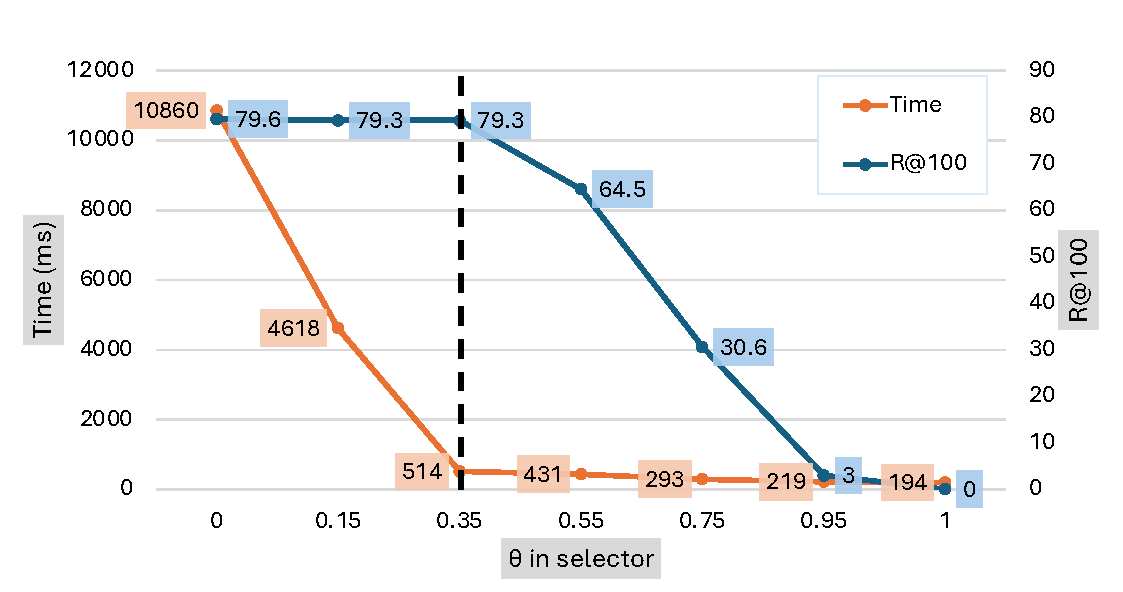
\includegraphics[width=0.6\linewidth]{Chapter5/Figures/theta_time.pdf}
    \caption{$\theta$ in the selector of RelQ-Former.}
    \label{fig:theta_time}
\end{figure}


\begin{table}[t]\small
    \centering
    \caption{Ablation study of RelQ-Former with different numbers of layers.}
    \resizebox{0.63\linewidth}{!}{
    \begin{tabular}{ccccccc}
        \toprule[1.5pt]
        ~ & \multicolumn{6}{c}{Predicate Classification} \\
        \cmidrule{2-7}
        Layer Num & R@20 & mR@20 & R@50 & mR@50 & R@100 & mR@100 \\
        \midrule[1pt]
        1 & 47.1 & 30.6 & 60.4 & 41.8 & 68.6 & 50.9 \\
        2 (Ours) & 55.1 & 39.2 & 70.6 & 53.8 & 79.3 & 63.8 \\
        4 & 55.1 & 39.5 & 70.7 & 54.0 & 79.8 & 64.1 \\
        6 & 54.2 & 38.5 & 69.4 & 52.8 & 78.3 & 62.8 \\
    \bottomrule[1.5pt]
    \end{tabular}
    }
    \label{tab:ablation_rel_q_former_layer}
\end{table}


\begin{table}[t]
    \centering
    \caption{Results on GQA: PredCls subtask in  closed- and open-set scenarios.}
    \resizebox{0.7\linewidth}{!}{
    \begin{tabular}{lcccc}
    % \hline
    \toprule[1.5pt]
        ~ & \multicolumn{2}{c}{Closed-set} & \multicolumn{2}{c}{Open-set (base:novel=7:3)} \\
        \cmidrule{2-5}
        Method & R/mR@50 & R/mR@100 & R/mR@50 & R/mR@100\\
        \midrule[1pt]
        SHA+GCL~\cite{dong2022stacked} & 41.0/42.7 & 42.7/44.5 & ~--~/~--~ & ~--~/~--~ \\
        OpenPSG & 46.2/44.1 & 48.3/45.8 & 23.6/22.7 & 26.2/25.0 \\
    % \hline
    \bottomrule[1.5pt]
    \end{tabular}
    }
    \label{tab:rebuttal_gqa}
\end{table}


\begin{table}[!ht]
    \centering
    \caption{Results on PSG: SGDet subtask in the open-set scenario.}
    \resizebox{0.8\linewidth}{!}{
    \begin{tabular}{lccc}
    \toprule[1.5pt]
        Method & R/mR@20 & R/mR@50 & R/mR@100\\
        \midrule[1pt]
        OpenPSG & 25.9/20.9 & 31.6/24.0 & 36.7/25.4 \\
        multi-division & \normalsize{26.4}\footnotesize{$\pm$0.7}\normalsize{/21.5}\footnotesize{$\pm$0.6} & \normalsize{31.4}\footnotesize{$\pm$0.4}\normalsize{/24.1}\footnotesize{$\pm$0.4} & \normalsize{36.5}\footnotesize{$\pm$0.4}\normalsize{/25.7}\footnotesize{$\pm$0.3} \\
        fuse G and J & 26.3/21.2 & 32.0/24.6 & 37.2/26.3 \\
    \bottomrule[1.5pt]
    \end{tabular}
    }
    \label{tab:rebuttal_psg}
\end{table}


\noindent \textbf{Effect of $\theta$ in the selector of RelQ-Former.}
To select the optimal $\theta$ to balance model performance and efficiency, we experiment with different $\theta$ parameters for the selector.
As shown in Fig.~\ref{fig:theta_time}, as $\theta$ increases from 0.0 to 0.35, the time required per image decreases rapidly, whereas there is no significant change as $\theta$ increases from 0.35 to 1.0.
At the same time, as $\theta$ rises from 0.0 to 0.35, there is only a minor decline in model performance; however, beyond 0.35, the performance of the model begins to decrease rapidly.
Therefore, to balance performance and efficiency, we select $\theta = 0.35$, thus ensuring a short average processing time for an image while maintaining high performance.


\noindent \textbf{Number of layers in RelQ-Former.}
To determine the number of layers for RelQ-Former, we conduct experiments with different numbers of layers, and the results are shown in Tab.~\ref{tab:ablation_rel_q_former_layer}.
When we increase the number of layers from 1 to 2, the model performance clearly improves, with R@100 increasing by 10.7\% and mR@100 by 12.9\%.
However, when the number of layers increases from 2 to 4, the model performance only sees a minimal improvement, with R@100 increasing by 0.5\% and mR@100 by 0.3\%.
Further increasing the number of layers from 4 to 6 leads to a slight decrease in model performance.
Considering that RelQ-Former requires a balanced layer number to extract features and learn relations without overwhelming computation for all possible subject-object pairs, i.e., $N \times (N-1)$ pairs.
Therefore, a layer number of 2 is the optimal choice for balancing performance and efficiency.



\noindent \textbf{Impact of different data divisions on the results.}
We conduct 5 random divisions of the base and novel classes in the PSG dataset and show that the results (mean and variance in Tab.~\ref{tab:rebuttal_psg}: multi-division) are rather stable, attesting to the robustness of our method.

\noindent \textbf{Fusion of generation and judgement instructions.}
Judgement instruction is used by default, while generation instruction is a variant inspired by~\cite{zhang2023simple} for comparison.
They are not combined in this chapter, but we can simply fuse their outputs using the inference fusion method in \cite{zhou2023hilo, zhou2023vlprompt}, the results in Tab.~\ref{tab:rebuttal_psg} (fuse G and J) show slight improvement (+0.5\% in R@100) but also come with double computation cost.


\section{Instructions used in Relation Query Transformer}
\label{sec:instruction_rel_q_former}
We introduce the instructions used in the relation query former (Sec.~4.2).
To prevent the model from overfitting to a particular type of instruction during training, following ~\cite{liu2024visual, dai2024instructblip, yu2023towards}, we design 10 different variations for each category of instruction.
During training, one is randomly selected from these 10 options for use, whereas for inference, only the first one is chosen for evaluation.

\subsection{Instructions for Pair Feature Extraction Query.}

\begin{lstlisting}[language=Python]
# {subject} is the category name of subject.
# {object} is the category name of object.
instructions_for_feat_query = [
    "Please extract features for the {subject}-{object} pair based on the whole visual features of the image and the masks of the {subject} and {object}.",
    "Based on the image's holistic visual features and the masks of both {subject} and {object}, please derive the features of the {subject}-{object} pair.",
    "Utilizing the total visual features of the image, along with the {subject} and {object} masks, please identify the features of the {subject}-{object} pair.",
    "By considering the comprehensive visual features of the image and the respective masks of the {subject} and {object}, please isolate the features specific to the {subject}-{object} pair.",
    "Taking into account the global visual features of the image and the masks designated for the {subject} and {object}, please extract the particular features of the {subject}-{object} pair.",
    "Leveraging the entire visual features of the image as well as the masks for the {subject} and {object}, please delineate the features corresponding to the {subject}-{object} pair.",
    "Drawing on the overall visual features of the image and the masks of the {subject} and {object}, please ascertain the features for the {subject}-{object} pair.",
    "By harnessing the full visual features of the image along with the masks of the {subject} and {object}, please identify the distinctive features of the {subject}-{object} pair.",
    "With reference to the comprehensive visual features of the image and the masks for the {subject} and {object}, please extract the respective features of the {subject}-{object} pair.",
    "Considering the total visual features of the image and the defined masks for the {subject} and {object}, please determine the specific features of the {subject}-{object} pair.",
]
\end{lstlisting}

\subsection{Instructions for Relation Existence Estimation Query.}

\begin{lstlisting}[language=Python]
# {subject} is the category name of subject.
# {object} is the category name of object.
instructions_for_exist_query = [
    "Based on the visual features of the entire image and the masks for the {subject} and {object}, estimate whether there is a relation between the {subject} and {object}.",
    "Considering the holistic visual features of the image and the masks of the {subject} and {object}, determine whether a relation exists between the two entities.",
    "Utilizing the complete visual features of the image along with the {subject} and {object} masks, assess whether there is a relation between the {subject} and {object}.",
    "Given the overall visual features of the image and the masks for the {subject} and {object}, evaluate whether a relation exists between the {subject} and {object}.",
    "By analyzing the entire visual features of the image and the masks of the {subject} and {object}, ascertain whether there is a relation between the {subject} and {object}.",
    "With the comprehensive visual features of the image and the masks for both {subject} and {object}, deduce whether there is a relation between the {subject} and {object}.",
    "Reflecting on the total visual features of the image and the masks applied to the {subject} and {object}, gauge whether there is a relation between the {subject} and {object}.",
    "Considering the full visual features of the image and the masks of the {subject} and {object}, infer whether a relation exists between the {subject} and {object}.",
    "Leveraging the overall visual features of the image and the masks designated for the {subject} and {object}, identify whether there is a relation between the {subject} and {object}.",
    "By examining the entire visual features of the image and the masks for the {subject} and {object}, predict whether there is a relation between the {subject} and {object}.",
]
\end{lstlisting}


\section{Instructions used in Multimodal Relation Decoder}
\label{sec:instruction_rel_decoder}
We introduce the instructions used in the multimodal relation decoder (Sec.~4.3).
Same as Sec.~\ref{sec:instruction_rel_q_former}, to avoid model overfitting to a particular type of instruction during training, we design 10 different variations for each type of instruction.
During training, one is randomly selected from these 10 options for use, whereas for inference, only the first one is chosen for evaluation [39].

\subsection{Generation Instructions.}

\begin{lstlisting}[language=Python]
# {subject} is the category name of subject.
# {object} is the category name of object.
instruction_for_generation = [
    "Please determine what the relation is between {subject} and {object}.",
    "Please ascertain the relation between the {subject} and {object}.",
    "Please identify what relations exists between the {subject} and {object}.",
    "Please decide what kind of relation is present between the {subject} and the {object}.",
    "Please deduce the relation between the {subject} and the {object}.",
    "Please establish what the relation is between the {subject} and {object}.",
    "Please clarify the relation between the {subject} and {object}.",
    "Please determine the type of relation existing between the {subject} and the {object}.",
    "Please pinpoint the kind of relation between the {subject} and {object}.",
    "Please evaluate what the relation is between the {subject} and the {object}.",
]
\end{lstlisting}

\subsection{Judgement Instructions.}

\begin{lstlisting}[language=Python]
# {subject} is the category name of subject.
# {object} is the category name of object.
# {relation} is the category name of relation.
instructions_for_judgement = [
    "Please judge between {subject} and {object} whether there is a relation {relation}.",
    "Please determine if there exists a relation between the {subject} and {object}, termed {relation}.",
    "Please ascertain whether there is a relation between the {subject} and {object}, identified as {relation}.",
    "Please evaluate if a relation between the {subject} and {object} can be classified as {relation}.",
    "Please judge whether there is a relation between the {subject} and {object} referred to as {relation}.",
    "Please decide if there is a relation between the {subject} and {object} denoted as {relation}.",
    "Please establish whether there is a relation between the {subject} and {object}, described as {relation}.",
    "Please conclude whether a relation exists between the {subject} and {object}, designated as {relation}.",
    "Please investigate whether there is a relation between the {subject} and {object}, recognized as {relation}.",
    "Please analyze if there exists a relation between the {subject} and {object}, characterized as {relation}.",
]
\end{lstlisting}

